Riprenderei appunti di Russo e basta. Riportiamo cmq quello che dice lei.
Ci sono quattro principi base nella relatività.
\begin{itemize}
    \item Ogni legge fisica è invariante in ogni sistema di riferimento inerziale.
    \item Energia, impulso, momento angolare in ogni sistema fisica isolato si conservano.
    \item La velocità della luce è la stessa in ogni sistema di riferimento.
    \item Il tempo non è invariante (assoluto).
    \item I primi due sono legati alla meccanica classica, gli ultimi due alla relatività. Da ciò ne segue che le trasformazioni galileiane non valgono più, e al loro posto ci sono le trasformazioni di Lorentz. Nel limite $\beta\ll1$ le trasformazioni di Lorentz diventano quelle di Galileo.
\end{itemize}
\subsection{Trasformazioni di Lorentz}
\begin{itemize}
    \item Definiamo i quadrivettori come $A=(a_0,a_i)=(a_0,\vec a)$, con $a_0$ componente temporale e $a_i$ componente spaziale.
    \item Definiamo il prodotto scalare tra quadrivettori come $\tilde A\tilde B =a_0b_0-a_ib_i$. Questo prodotto è invariante sotto trasformazioni di Lorentz.
    \item Se consideriamo un sistema di riferimento $S$ e un altro $S'$, con $S'$ che si muove rispetto a $S$ con velocità $v$ lungo l'asse $x$, allora le trasformazioni di Lorentz sono date da:
    \begin{equation*}
        \mqty(a'_0 \\\xmat*{a'}{3}{1})= 
        \underbrace{\begin{pmatrix}
            \mqty{\gamma & -\beta\gamma & 0 & 0 \\ -\beta\gamma & \gamma &0&0 \\ 
            0 & 0 & 1 & 0 \\ 
            0 & 0 & 0 & 1 }
        \end{pmatrix}}_{=L(\beta)}
        \mqty(a_0 \\\xmat*{a}{3}{1})= 
        \mqty(\gamma a_0-\beta\gamma a_1\\-\beta\gamma a_0+\gamma a_1\\a_2\\a_3)\implies 
        \begin{cases}
            ct'=\gamma(ct-\beta x) \\
            x'=\gamma(x-\beta ct)
        \end{cases}
    \end{equation*}
    Una proprietà importante è $L(\beta)^{-1}=L(-\beta)$, da cui ne segue che per invertire le trasformazioni di Lorentz basta scambiare variabile con indice con quelle senza e $\beta\to-\beta$.
    \item Che si ha al limite non relativistico? Supponiamo $\beta\ll1\implies\gamma\approx1+\frac{\beta^2}{2}\approx1$. Ne segue per il tempo che
    \begin{equation*}
        ct'=\qty(1+\frac{\beta^2}2)(ct-\beta x) \approx ct-\beta x + \frac{\beta^2}2ct\approx ct\implies t'=t 
    \end{equation*}
    e per lo spazio che 
    \begin{equation*}
        x'=\qty(1+\frac{\beta^2}2)(x-\beta ct)\approx x-\beta ct\implies x'= x - vt
    \end{equation*}
    \item Se il moto non è solo lungo $x$, allora dobbiamo considerare $\vec\beta=\frac{\vec v} c$ e 
    \begin{equation*}
        \begin{cases}
            ct'=\gamma(ct-\beta x_\parallel) \\
            x'_\parallel=\gamma(x_\parallel-\beta ct)\\
            \vec x_\perp'=\vec x_\perp
        \end{cases}
    \end{equation*}
    \item Dimostriamo che il prodotto scalare è invariante. Sia $A=(a_0,\vec a)$ e $B=(b_0,\vec b)$. Calcoliamo $A'\cdot B'$.
    \begin{equation*}
        A'\cdot B'=a_0'b_0'-\vec a'\cdot\vec b'=\gamma^2(a_0-\beta a_1)(b_0-\beta b_1)-\gamma^2(a_1-\beta a_0)(b_1-\beta b_0)-a_2b_2-a_3b_3=\dots=A\cdot B
    \end{equation*}
\end{itemize}
Vediamo alcune conseguenze in high energy physics.
\begin{itemize}
    \item La contrazione delle lunghezze. Consideriamo un oggetto di lunghezza $L$ che si muove con velocità $v$. Supponiamo che il sistema solidale ad esso sia $S'$ e la lunghezza misurata sia $d'=x_2'-x_1'$ che avviene simultaneamente quindi $t_2=t_1$. Se trasformiamo otteniamo $d'=x_2'-x_1'=\gamma(x_2-\beta ct_2)-\gamma(x_1-bct_1)=\gamma(x_2-x_1)-\gamma\beta c(t_2-t_1)=\gamma(x_2-x_1)=d\implies d'=\gamma d$. Ne segue che la lunghezza misurata da un osservatore in moto è contratta di un fattore $\gamma$, e la lunghezza propria, misurata nel sistema solidale all'oggetto è la massima possibile.
    \item La dilatazione temporale. Consideriamo due eventi che avvengono nello stesso punto nello spazio, ma in tempi diversi. Se trasformiamo otteniamo $c\Delta t=c(t_2-t_1)=\gamma c(t_2'-t_1')+\beta \gamma (x_2'-x_1')=\gamma c\Delta t'$. Ne segue che il tempo misurato da un osservatore in moto è dilatato di un fattore $\gamma$, e il tempo proprio, misurato nel sistema solidale all'oggetto è il minimo possibile. Da ciò si hanno varie conseguenze.
\end{itemize}
Slide su esperimento di Conversi, Pancini, Piccioni (CPP) sui pioni e muoni.
\begin{itemize}
    \item Nel 1912 Hess scoprì i raggi cosmici. Nel 1932 Anderson scoprì i positroni, predetti da Dirac nel 1928 (già discussa).
    \item Nel 1935 Yukawa introdusse la teoria delle interazioni forti, predicendo una massa mediatrice di $\sim 100$ MeV. Il mesone di Yukawa doveva decadere in elettrone e netruino con tempo di decadimento di $\sim1\mu$s. Nel 1937 si scoprì il mesotrone (Anderson), con una massa di $110$ MeV, associata alla particella di Yukawa. Nel 1940 si studiò assorbimento e decadimento delle proprietà di assorbimento del mesone di Yukawa.
    \item Il decadimento del mestrone (che in realtà è un $\mu$) fu studiato diverse volte. Nel 1940 si osservò il suo decadimento in positroni; nel 1941 ci fu una misura da Rasetti che ottenne $\tau=(1.5\pm0.3)\mu$s. Nel 1941 Piccioni e Conversi decisero di lavorare assieme e migliorare la precisione nella misura del tempo di decadimento (del mesone di Yukawa).
    \item Nel 1939 Montgomery fece un esperimento (\autoref{fig:montgomery}) per misurare il decadimento del $\mu$
    \begin{figure}[h]
        \centering
        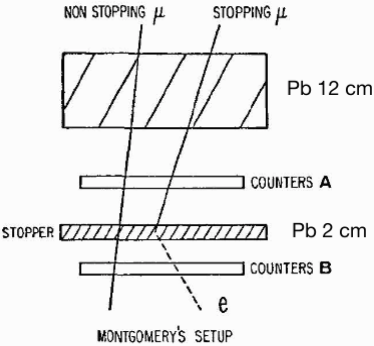
\includegraphics[width=0.6\textwidth]{immagini/fig_montgomery.png}
        \caption{}
        \label{fig:montgomery}
      \end{figure}
      \item pippo
\end{itemize}